\documentclass[12pt,a4paper]{article}
\usepackage{float}
\usepackage{commons/course}


%\hidesolutions

\شروع{نوشتار}

\سربرگ{تمرین اول}{}{ شمارش،مقدمات احتمال،احتمال شرطی،استقلال}{گردآورندگان: محمدرضا احمدخانی، سروش تسلیمی، علیرضا اکبری}


\section*{
شمارش و مقدمات احتمال
}

\مسئله{‌مجموعه بازی*}

تعداد زیرمجموعه های k عضوی از مجموعه ی $\{1, 2, 3, ..., n\}$ را بیابید که هیچ دو عضوی از آن متوالی نباشند.


\مسئله{‌رنگ بازی*}
فرض کنید متغیر تصادفی X از یک توزیع
$
Binomial(n, p)
$
می‌آید.
\subsection*{الف}
اگر
$
p < \alpha < 1
$
، با استفاده از نابرابری مارکوف، یک کران بالا برای 
$
P(X \ge \alpha n)
$
بیاید. 

\subsection*{ب}
مقدار عددی این کران را برای 
$
p = \frac{1}{2}
$
و
$
\alpha = \frac{3}{4}
$
بیابید.



\مسئله{‌جرئت یا حقیقت؟}

فرض کنید در یک پرواز، موتور های هواپیما به احتمال $1 - p$ خراب می شوند و احتمال خرابی هر موتور از موتور های دیگر مستقل است.اگر یک هواپیما برای پرواز نیاز داشته باشد تا بیشتر از نصف موتور هایش سالم باشند،به ازای چه مقادیری از $p$ یک هواپیما با 5 موتور را به یک هواپیما با 3 موتور ترجیح می دهید؟


\مسئله{‌جایگشت}
صورت کلی مسئله 

\subsection*{الف}
صورت بخش اول 

\subsection*{ب}
صورت بخش دوم 

\subsection*{ج}
صورت بخش سوم

\section*{
احتمال شرطی ، استقلال
}

\مسئله{‌بچه چیه؟}
ثابت کنید متغیرهای
$ X_1 $
, ... ,
$ X_n $
مستقلند اگر و تنها اگر تابع توزیع توام آن‌ها به شکل زیر قابل بیان باشد.
\begin{center}
	$f( x_1, x_2, ..., x_n ) = \prod_{i=1}^n g_i(x_i)$
\end{center}
$ g_i $
تابعی مثبت است.



\مسئله{‌فروشگاه قطعات ماشین*}
توزیع \lr{Pareto}  با دو پارامتر $\alpha$ و $x_m$ مشخص می‌شود. می‌دانیم که $x_1$، $x_2$، ... و $x_n$ داده‌هایی رندوم از توزیع \lr{Pareto} با $\alpha  >2$ هستند. خصوصیات توزیع \lr{Pareto} داده‌هایمان در ادامه آورده شده است:
$$PDF:\ \frac{\alpha{x_m}^\alpha}{x^{\alpha+1}},\ \alpha>2,\ x_m>0,\ x\geq x_m$$
$$CDF:\ 1 - (\frac{x_m}{x})^\alpha$$
$$Mean:\ \frac{\alpha x_m}{\alpha - 1}$$
$$Variance:\ \frac{\alpha {x_m}^2}{(\alpha - 1)^2(\alpha - 2)}$$

\subsection*{الف}
با استفاده از تخمین‌گر \lr{MLE} پارامترهای $\alpha$ و $x_m$ را تخمین بزنید.

\subsection*{ب}
وضعیت \lr{unbiased} بودن و \lr{consistent} بودن تخمین‌گر \lr{MLE} برای $x_m$ را مشخص کنید. 
\\(راهنمایی: اگر n متغیر تصادفی \lr{iid} از توزیعی با $CDF:\ F$ باشند، مینیموم این متغیرها متغیر تصادفی‌ای با $CDF:\ 1-(1-F)^n$ است)



\مسئله{‌توپ بازی*}
\textbf{جدول
\lr{t}
در ادامه آمده است.}

اداره هواشناسی یک شهر، ۴ دستگاه سنجش آلودگی هوا را در یک منطقه قرار داده است. فرض کنید شاخص آلودگی هوا در این منطقه ثابت است اما این دستگاه‌ها دقیق نیستند و شاخص را با کمی نویز گزارش می‌دهند. در یک روز نسبتا آلوده، مقادیر گزارش شده توسط این ۴ دستگاه به شرح زیر است.
$$152, 148, 153, 153$$

\subsection*{الف}
با کمک داده‌های جمع آوری شده، یک بازه اطمینان ۹۵ درصد برای شاخص آلودگی هوا در آن ایستگاه ارائه دهید.

\subsection*{ب}
در صورتی که شاخص آلودگی هوا از ۱۵۰ بیشتر باشد، هوا در شرایط ناسالم برای تمامی گروه‌ها قرار می‌گیرد. عده‌ای از دانشمندان معتقدند که میانگین شاخص آلودگی ۱۵۰ بوده بنابراین هوای این منطقه ناسالم نیست، در حالی که عده‌ی دیگری معتقند میانگین شاخص آلودگی به طور معنی‌داری از ۱۵۰ بیشتر بوده و هوا ناسالم است. برای بررسی این افراد یک آزمون فرض طراحی کنید. فرض صفر و فرض دیگر این آزمون را بیان کرده و سپس مشخص کنید آیا با سطح اهمیت 
$0.05$
می‌توان فرض صفر را رد کرد یا خیر.

\subsection*{پ}
برای کاهش خطای نوع اول، باید سطح اهمیت را افزایش دهیم یا کاهش؟ برای کاهش خطای نوع دوم چه طور؟

\begin{figure}[H]
    \centering
    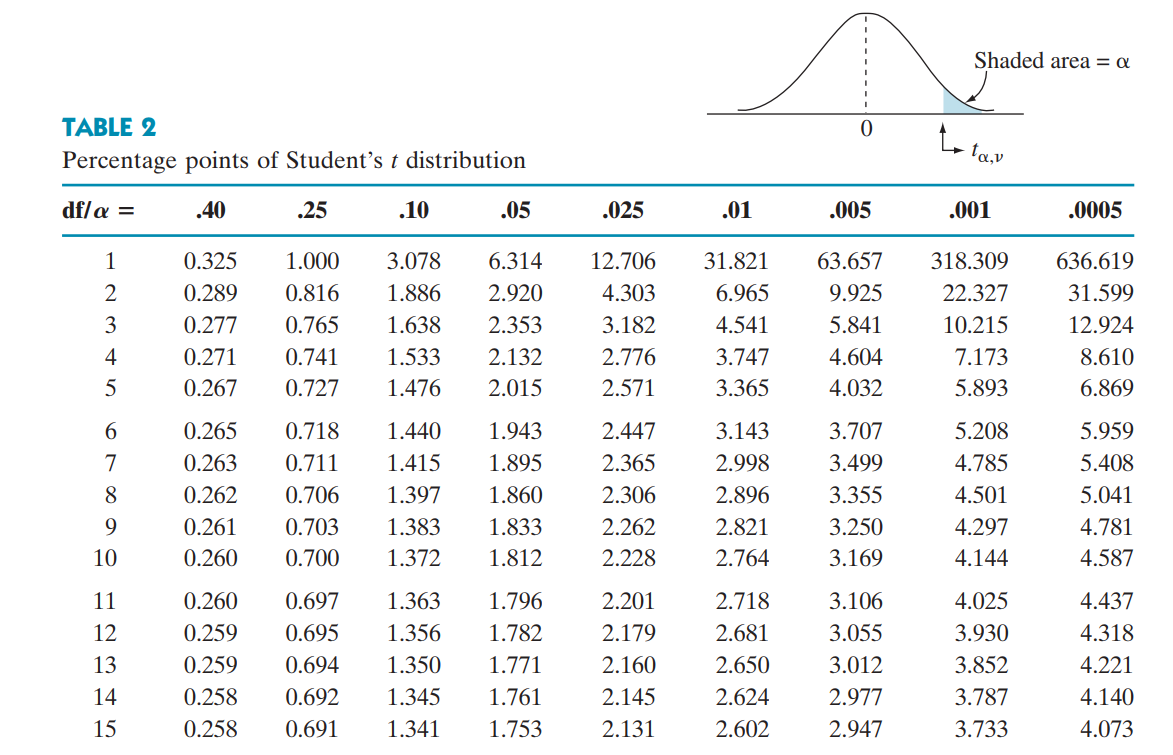
\includegraphics[width=7in,height = 5in]{tStudent}
\end{figure}



\مسئله{‌بادکنک بازی}

عمر چرخ یک ماشین مشخصی از یک توزیع نرمال با میانگین 34000 کیلومتر و انحراف از معیار 4000 کیلومتر پیروی می کند.

\subsection*{الف}
احتمال اینکه چرخ این ماشین بیش از 40000 کیلومتر عمر کند چقدر است؟
\subsection*{ب}
احتمال اینکه چرخ این ماشین بین 30000 تا 35000 کیلومتر عمر کند چقدر است؟
\subsection*{ج}
فرض کنید به ما گقته شده است که چرخ این ماشین تا الان 30000 کیلومتر عمر کرده است.احتمال اینکه 10000 کیلومتر دیگر عمر کند چقدر است.






\مسئله{‌سکه بازی*}

فزض کنید $f(x) = 0$ تابع توزیع یک متغیر تصادفی نرمال با میانگین $\mu$ و واریانس $\sigma ^ 2$ باشد.نشان دهید که $f''(x) = 0$ وقتی که $x$ برابر با مقادیر $\mu - \sigma$ و $\mu + \sigma$ باشد.



\مسئله{
این کارا آخر عاقبت نداره!
\پاورقی{
Gambler's Ruin
}
(
برای علاقه‌مندان
)
}

صورت کلی مسئله 

\subsection*{الف}
صورت بخش اول 

\subsection*{ب}
صورت بخش دوم 

\subsection*{ج}
صورت بخش سوم





\begin{flushleft}
	موفق باشید :)
\end{flushleft}



\پایان{نوشتار}
